\subsection{Calculating upper limits}
\label{ssec:upper_limits}

Given no evidence for \ac{BNS} or \ac{NSBH} coalescences during \ac{O1}, we seek to place an upper limit
on the astrophysical rate of such events.
The expected number of observed events $\Lambda$ in a given analysis can be
related to the astrophysical rate of coalescences for a given source $R$ by
%
\begin{linenomath*}
\begin{equation}
    \Lambda = R { \langle VT \rangle}.
\end{equation}
\end{linenomath*}
%
Here, $\langle VT \rangle$ is the space-time volume that the detectors are sensitive
to---averaged over space, observation time, and the parameters of the source population
of interest. The likelihood for finding zero observations in the data $s$ follows the
Poisson distribution for zero events $p (s \, | \, \Lambda) = e^{-\Lambda}$. We use
the notation of $\mathcal{L} (s \, | \, \Lambda)$ for likelihoods. Bayes' theorem then
gives the posterior for $\Lambda$
%
\begin{linenomath*}
\begin{equation}
    p (\Lambda \, | \, s) \propto \pi (\Lambda) e^{-\Lambda},
\label{eq:lambdapost}
\end{equation}
\end{linenomath*}
%
where $p(\Lambda)$ is the prior on $\Lambda$. We switch notation for posteriors
to be $\mathcal{P}(\Lambda \, | \, s)$ and priors to be noted as $\pi(\Lambda)$.

Searches of Initial \ac{LIGO} and Initial Virgo data used a uniform prior on
$\Lambda$~\citep{Colaboration:2011np} but included prior information from previous searches. 
For the \ac{O1} \ac{BBH} search, however, a Jeffreys prior of
$p(\Lambda) \propto 1/\sqrt{\Lambda}$ for the Poisson likelihood was used~\citep{Farr:2013yna,Abbott:2016nhf,TheLIGOScientific:2016pea}.
A Jeffreys prior has the convenient property that the resulting posterior is invariant under a change in parametrization. 
However, for consistency with past BNS and NSBH results we will primarily use a uniform prior, and note that a Jeffreys
prior generally predicts a rate upper limit that is $\sim 40$\% smaller. 
We do not include additional prior information because the sensitive $\langle VT \rangle$ from 
all previous runs is an order of magnitude smaller than that of \ac{O1}.
We estimate $\langle VT \rangle$ by adding a large number of
simulated waveforms sampled from an astrophysical population into the data. 
These simulated signals
are recovered with an estimate of the FAR using the offline analyses.
Monte-Carlo integration methods are then utilized to estimate
the sensitive volume to which the detectors can recover gravitational-wave signals
below a chosen FAR threshold, which in this paper we will choose to be $0.01 \mathrm{yr}^{-1}$.
This threshold is low enough that only signals that are likely to be true events are counted as found, and we 
note that varying this threshold in the range 0.0001--1~yr$^{-1}$ only changes the calculated $\langle VT \rangle$ 
by about $\pm 20\%$.

Calibration uncertainties lead to a difference between the amplitude of simulated
waveforms and the amplitude of real waveforms with the same luminosity distance $d_L$.
During \ac{O1}, the $1\sigma$ uncertainty in the strain amplitude was 6\%, resulting
in an 18\% uncertainty in the measured $\langle VT \rangle$. Results presented here
also assume that injected waveforms are accurate
representations of astrophysical sources. We use a time-domain, aligned-spin,
post-Newtonian point-particle approximant to model \ac{BNS}
injections~\citep{Buonanno:2009zt}, and a time-domain, effective-one-body waveform
calibrated against numerical relativity to model \ac{NSBH}
injections~\citep{Pan:2013rra,Taracchini:2013rva}. Waveform differences between these models and
the offline search templates are therefore including in the calculated $\langle VT \rangle$. 
The injected NSBH waveform model is not calibrated at high mass ratios
($m_1/m_2 >8$), so there is some additional modeling uncertainty for large-mass NSBH
systems. The true sensitive volume $\langle VT \rangle$  will also be smaller if the effect of
tides in \ac{BNS} or \ac{NSBH} mergers is extreme. However, for most scenarios
the effects of waveform modeling will be smaller than the
effects of calibration errors and the choice of prior discussed above. 

The posterior on $\Lambda$ (Eq.~\ref{eq:lambdapost}) can be reexpressed as a joint
posterior on the astrophysical rate $R$ and the sensitive volume  $\langle VT \rangle$
\begin{linenomath*}
\begin{equation}
    \mathcal{P}(R, \langle VT \rangle \, | \, s) \propto \pi(R, \langle VT \rangle) \, e^{-R \langle VT \rangle}.
\end{equation}
\end{linenomath*}
%
The new prior can be expanded as $\pi(R, \langle VT \rangle) = \pi(R \, | \, \langle VT \rangle) \pi(\langle VT \rangle)$. 
For $\pi(R \, | \, \langle VT \rangle)$, we will either use a uniform prior on $R$ or a prior proportional to the 
Jeffreys prior $1/\sqrt{R \langle VT \rangle}$. As with Refs.~\citep{Abbott:2016nhf, Abbott:2016drs, TheLIGOScientific:2016pea}, 
we use a log-normal prior on $\langle VT \rangle$
%
\begin{linenomath*}
\begin{equation}
\pi(\langle VT \rangle) = \ln \mathcal{N}(\mu, \sigma^2),
\end{equation}
\end{linenomath*}
%
where $\mu$ is the calculated value of $\ln\langle VT \rangle$ and $\sigma$ represents the fractional uncertainty
in $\langle VT \rangle$. Below, we will use an uncertainty of
$\sigma=18\%$ due mainly to calibration errors.

Finally, a posterior for the rate is obtained by marginalizing over $\langle VT \rangle$
%
\begin{linenomath*}
\begin{equation}
\mathcal{P}(R \, | \, s) = \int d\langle VT \rangle\, \mathcal{P} (R, \langle VT \rangle \, | \, s).
\label{eq:posterior}
\end{equation}
\end{linenomath*}
%
The upper limit $R_c$ on the rate with confidence $c$ is then given by the solution to
%
\begin{linenomath*}
\begin{equation}
\label{eq:upperlimit}
\int_0^{R_c} dR\, \mathcal{P}(R \, | \, s) = c.
\end{equation}
\end{linenomath*}

For reference, we note that in the limit of zero uncertainty in $\langle VT \rangle$,
the uniform prior for $\pi(R | \langle VT \rangle)$ gives a rate upper limit of
%
\begin{linenomath*}
\begin{equation}
R_c = \frac{ -\ln(1-c) }{ \langle VT \rangle },
\end{equation}
\end{linenomath*}
%
corresponding to $R_{90\%} = 2.303/\langle VT \rangle$ for a 90\% confidence upper
limit~\citep{Biswas:2007ni}. For a Jeffreys prior on $\pi(R | \langle VT \rangle)$, this upper limit is
%
\begin{linenomath*}
\begin{equation}
R_c = \frac{ [{\rm erf}^{-1}(c)]^2 }{ \langle VT \rangle },
\end{equation}
\end{linenomath*}
%
corresponding to $R_{90\%} = 1.353/\langle VT \rangle$ for a 90\% confidence upper limit.


\subsection{BNS rate limits}
\label{ssec:bns_rate_limits}

\begin{figure}[t]
   \centering
   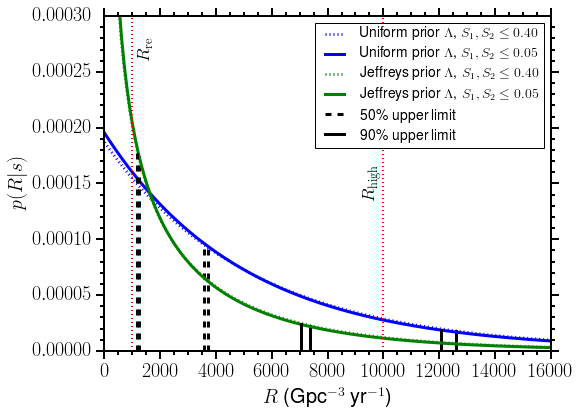
\includegraphics[width=\columnwidth]{figs/chapter3/figure3.png} 
   \caption{Posterior density on the rate of \ac{BNS} mergers calculated using the \pycbc\ analysis.
   Blue curves represent
   a uniform prior on the Poisson parameter $\Lambda = R \langle VT \rangle$, while
   green curves represent a Jeffreys prior on $\Lambda$. The solid (low spin population)
   and dotted (high spin population) posteriors almost overlap. The vertical dashed and
   solid lines represent the 50\% and 90\% confidence upper limits respectively for each
   choice of prior on $\Lambda$. For each pair of vertical lines, the left line is the 
   upper limit for the low spin population and the right line is the upper limit for the high
   spin population. Also shown are the realistic $R_{\rm re}$ and high end
   $R_{\rm high}$ of the expected \ac{BNS} merger rates identified in Ref.~\citep{Abadie:2010cf}.}
   \label{fig:bnspdf}
\end{figure}

\begin{figure}[t]
\centering
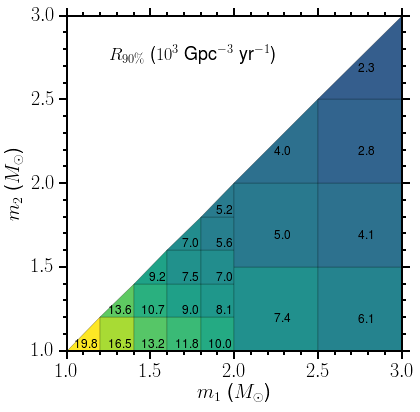
\includegraphics[width=1.0\textwidth]{figs/chapter3/figure4.png}
\caption{\label{fig:bns_ul_vs_mass} 90\% confidence upper limit on the \ac{BNS} merger rate as a function of the two component
masses using the \pycbc\ analysis. Here the upper limit for each bin is obtained assuming a \ac{BNS} population with masses distributed uniformly
within the limits of each bin, considering isotropic spin direction and dimensionless spin magnitudes uniformly
distributed in $[0, 0.05]$.}
\end{figure}

Motivated by considerations in Section \ref{sec:source_considerations}, we begin by
considering a population of \ac{BNS} sources with a narrow range of component
masses sampled from the normal distribution $\mathcal{N}(1.35M_\odot, (0.13M_\odot)^2)$
and truncated to remove samples outside the range $[1,3] M_{\odot}$. We consider
both a ``low spin'' \ac{BNS} population, where spins are distributed with uniform dimensionless
spin magnitude $\in [0, 0.05]$ and isotropic direction, and a ``high spin'' \ac{BNS}
population with a uniform dimensionless spin magnitude $\in [0, 0.4]$ and isotropic direction.
Our population uses an isotropic distribution of sky location and source orientation and chooses
distances assuming a uniform distribution in volume.
These simulations are modeled using a post-Newtonian waveform model, expanded using the
``TaylorT4'' formalism~\citep{Buonanno:2009zt}.
From this population we compute the space-time volume that Advanced \ac{LIGO} was
sensitive to during the O1 observing run. Results are shown for the measured $\langle VT\rangle$
in Table~\ref{tab:bns_ul_table} using a detection threshold of $\mathrm{FAR} = 0.01\, \mathrm{yr}^{-1}$.
Because the template bank for the searches use only aligned-spin \ac{BNS} templates with 
component spins up to 0.05, the \pycbc\ pipeline is 4\% more sensitive 
to the low-spin population than to the high-spin population.
The difference in $\langle VT\rangle$ between the two analyses is no larger than 5\%, which
is consistent with the difference in time analyzed in the two analyses. 
In addition, the calculated $\langle VT \rangle$
has a Monte Carlo integration uncertainty of $\sim1.5\%$ due to the finite number of injection
samples.

Using the measured $\langle VT \rangle$, the rate posterior and upper limit can be
calculated from Eqs.~\ref{eq:posterior} and~\ref{eq:upperlimit} respectively.
The posterior and upper limits are shown in Figure~\ref{fig:bnspdf} and depend
sensitively on the choice of uniform versus Jeffreys prior
for $\Lambda=R\langle VT \rangle$. However, they depend only weakly on the spin
distribution of the \ac{BNS} population and on the width $\sigma$ of the uncertainty
in $\langle VT \rangle$. For the conservative uniform prior on $\Lambda$ and an
uncertainty in $\langle VT \rangle$ due to calibration errors of 18\%, we find the
90\% confidence upper limit on the rate of \ac{BNS} mergers to be \MainBNSULLowSpin~Gpc$^{-3}$~yr$^{-1}$
for low spin and \MainBNSULHighSpin~Gpc$^{-3}$~yr$^{-1}$ for high spin using the values of $\langle VT \rangle$
calculated with \pycbc. These numbers can be compared to the upper limit 
computed from analysis of Initial \ac{LIGO} and Initial Virgo data~\citep{Colaboration:2011np}. 
There, the upper limit for $1.35$ -- $1.35 M_{\odot}$ non-spinning \ac{BNS} mergers is given 
as \SSixULNoSpin. The O1 upper limit is more than an order of magnitude lower than this previous upper limit.

To allow for uncertainties in the mass distribution of \ac{BNS} systems we also
derive 90\% confidence upper limits as a function of the \ac{NS} component masses.
To do this we construct a population of software injections with component masses
sampled uniformly in the range $[1, 3]M_{\odot}$, and an isotropic distribution
of component spins with magnitudes uniformly distributed in $[0, 0.05]$. We then bin
the \ac{BNS} injections by mass, and calculate $\langle VT \rangle$ and the associated 90\%
confidence rate upper limit for each bin. The 90\% rate upper limit for the conservative
uniform prior on $\Lambda$ as a function of component masses is shown in 
Figure~\ref{fig:bns_ul_vs_mass} for \pycbc. The fractional difference between the \pycbc\
and \gstlal\ results range from 1\% to 16\%.

\subsection{NSBH rate limits}
\label{ssec:nsbh_rate_limits}

\begin{figure}[t]
\centering
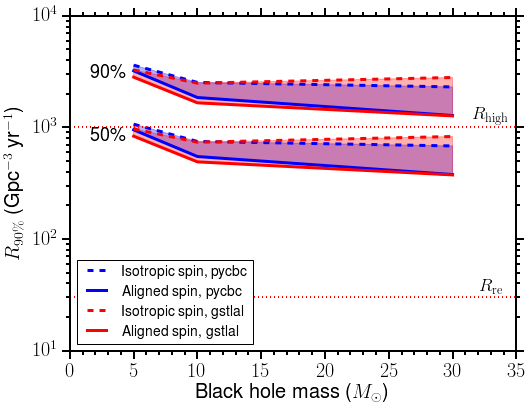
\includegraphics[width=1.0\textwidth]{figs/chapter3/figure5.png}
\caption{\label{fig:nsbh_ul_vs_mass} 50\% and 90\% upper limits on the \ac{NSBH} merger rate
as a function of the \ac{BH} mass using the more conservative uniform prior for the counts $\Lambda$. 
Blue curves represent the \pycbc\ analysis and red curves
represent the \gstlal\ analysis. The \ac{NS} mass is assumed to be $1.4M_\odot$. The spin magnitudes
were sampled uniformly in the range [0, 0.04] for \acp{NS} and [0, 1] for \acp{BH}. For the aligned
spin injection set, the spins of both the \ac{NS} and \ac{BH} are aligned (or anti-aligned) with the
orbital angular momentum. For the isotropic spin injection set, the orientation for the
spins of both the \ac{NS} and \ac{BH} are sampled isotropically. The isotropic spin distribution results
in a larger upper limit. Also shown are the realistic $R_{\rm re}$ and high end
$R_{\rm high}$ of the expected \ac{NSBH} merger rates identified in Ref.~\citep{Abadie:2010cf}.}
\end{figure}

Given the absence of known \ac{NSBH} systems and uncertainty in the \ac{BH} mass, we evaluate the
rate upper limit for a range of \ac{BH} masses. We use three masses that span the likely
range of \ac{BH} masses: $5M_\odot$, $10M_\odot$, and $30M_\odot$. For the \ac{NS} mass,
we use the canonical value of $1.4M_\odot$. We assume a distribution of \ac{BH} spin magnitudes
uniform in $[0,1]$ and \ac{NS} spin magnitudes uniform in $[0, 0.04]$.
For these three mass pairs, we compute upper limits for an isotropic spin distribution
on both bodies, and for a case where both spins are aligned or anti-aligned with the orbital angular momentum
(with equal probability of aligned vs anti-aligned).
Our NSBH population uses an isotropic distribution of sky location and source orientation and chooses
distances assuming a uniform distribution in volume. Waveforms are modeled
using the spin-precessing, effective-one-body model calibrated against numerical relativity
waveforms described in Ref.~\citep{Taracchini:2013rva,babak2016validating}.

The measured $\langle VT \rangle$ for a FAR threshold of $0.01 \mathrm{yr}^{-1}$ is given in Table~\ref{tab:nsbh_ul_table}
for \pycbc\. The uncertainty in the Monte Carlo integration of $\langle VT \rangle$ is 1.5\%--2\%. The corresponding 
90\% confidence upper limits are also given using the conservative 
uniform prior on $\Lambda$ and an 18\% uncertainty in $\langle VT
\rangle$. Analysis-specific differences in the limits range from 1\% to 20\%,
comparable or less than other uncertainties such as calibration.  
These results can be compared to the upper limits found for initial \ac{LIGO} and Virgo
for a population of $1.35M_\odot$--$5M_\odot$ \ac{NSBH} binaries with isotropic spin of
\SSixNSBHULFiveSpin at 90\% confidence~\citep{Colaboration:2011np}.
As with the \ac{BNS} case, this is an improvement in the upper limit of over an order of magnitude.

We also plot the 50\% and 90\% confidence upper limits from \pycbc\ and \gstlal\ as a function of mass in 
Figure~\ref{fig:nsbh_ul_vs_mass} for the uniform prior. The search is
less sensitive to isotropic spins than to (anti-)aligned spins due to two factors.
First, the volume-averaged signal
power is larger for a population of (anti-)aligned spin systems than for isotropic-spin systems.
Second, the search uses a template bank of (anti-)aligned spin systems, and thus loses sensitivity
when searching for systems with significantly misaligned spins.
As a result, the rate upper limits are less constraining
for the isotropic spin distribution than for the (anti-)aligned spin case.
